% !TeX root = dissertation.tex
\chapter{Optimized data movement in \hira}\label{chapter:vTask}

\aak{THIS IS THE UNFINISHED CHAPTER; PROCEED TO PAGE 63 FOR RELATED WORK.}

\hirafull works by interposing API calls invoked by the application in the
guest OS, and forwarding them to an \worker in the host, via
hypervisor-mediated transport. Typically, \workers are per-API (for modularity
and failure isolation between APIs and accelerators, and to support remote
resources) and per-guest (to preserve isolation between guests). Applications
that use multiple API frameworks will be associated with multiple API-servers,
one per framework. Previous chapters in this dissertation established the
efficacy of the \hirafull (\hira) technique for virtualizing API-controlled
Domain Specific Accelerators. This chapter considers a performance issue that
arises from the choice of interposing the user-space API: that of redundant
data movement in the virtualization stack.

Any virtualization scheme based on interposing the user-space API, burdens
applications that pipeline disparate DSA API frameworks with redundant data
movement. All inter-framework data movement must take place in the guest
application as that the only point where they share the same logical address
space. The left-hand side of Figure~\ref{fig:vtask_overview} illustrates this
scenario. Consider a guest application (\texttt{Guest Application} in the
figure) that pipelines functions from two API frameworks: \texttt{API-1}, and
\texttt{API-2}. When the first API framework function is invoked, the
associated data is copied from the \texttt{Guest Application} to
\texttt{API-Server-1}, and then to \texttt{Device-1}’s memory. Once the
function has finished executing on \texttt{Device-1}, the result is copied
first to \texttt{API-Server-1}, and then to the \texttt{Guest Application}.
Since we're considering a pipelined scenario, when the \texttt{Guest
  Application} invokes the function from \texttt{API-2}, the same data (i.e.,
the output of the \texttt{API-1 function}) will be copied from the
\texttt{guest application} to \texttt{API-server-2} and then to
\texttt{Device-2} to be processed.
\aak{Add note here about measured overhead. Is this a real problem?}

\begin{figure}[ht!]
  \centering
  \captionsetup{justification=centering,width=\linewidth}
  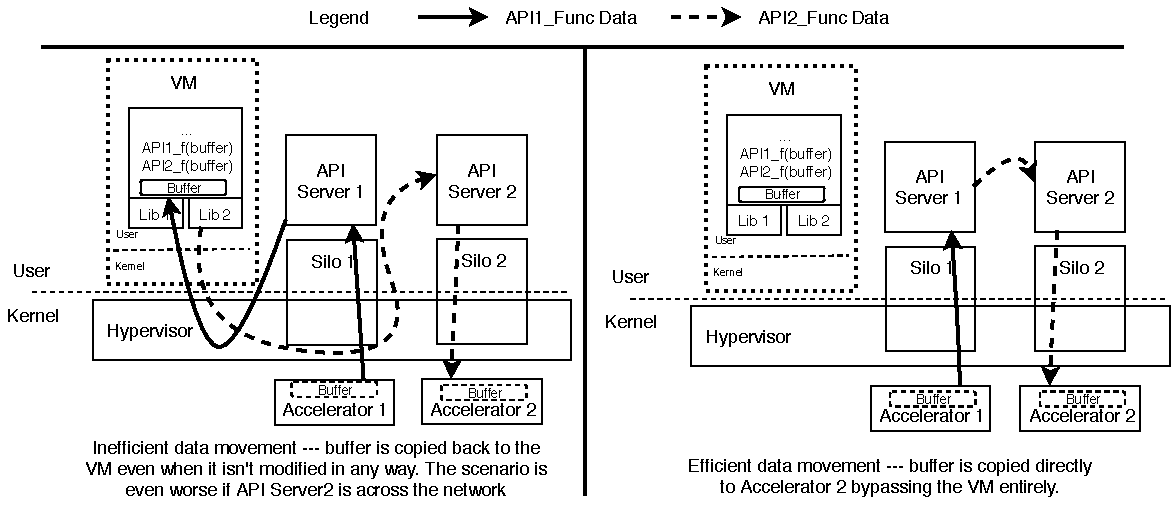
\includegraphics[width=\linewidth]{figures/vtask-overview.pdf}
  \caption{All data processed by multiple DSA API frameworks must pass through the guest application, leading to redundant data movement.}\label{fig:vtask_overview}
\end{figure}

The crux of the issue is that the guest application (and the virtualization
scheme's interposition library) is the only point in the constructed
software stack where the two API frameworks are in the same address space. At
all other points, the two API frameworks have no notion of the other's
existence. Such a design is typically desirable for maintaining isolation, and
to enable independent scaling, migration etc.

The right hand side of Figure~\ref{fig:vtask_overview} illustrates the desired
behavior in the scenario described before. As before, consider a guest
application that invokes functions from two API frameworks in a pipelined
fashion, i.e., the output of the function from the API1 framework is consumed
by a function from the API2 framework. In such a scenario, eliding movement of
data to and from the guest application would lead to improved performance.
Further optimization may also be possible: peer-to-peer data copy between the
devices if they are on the same machine, or by directly copying the data from
the first API-server on one remote machine to the second API-server on another
remote machine.

Given this overhead arises due to the introduction of virtualization,
this chapter explores techniques to eliminate it automatically, i.e., without
involving the end user.
In order to automatically eliminate the redundant data movement described in
the left side of Figure~\ref{fig:vtask_overview} when an application uses
multiple accelerators via API-remoting, the flow of data among these API calls
must be tracked. Keeping track of where the data flowed from and to, the
validity of different copies of the data (e.g., if the data is modified on the
accelerator, but hasn’t been copied back to the guest application), etc., will
enable the virtualization system to detect scenarios like the one presented in
the left side of Figure~\ref{fig:vtask_overview} and transform them to the one
shown on the right side of the figure instead.

Automatic detection and tracking of data movement among accelerator API
frameworks requires semantic understanding of the interposed API functions.
The API function annotations provided by \lapis allow us to identify parts of
the API that deal with the movement of data, the direction of movement, and the
actual data itself. This chapter describes vTask, an optimization for \AvA that
leverages \lapis annotations to orchestrate data movement among accelerators
virtualized with \hira in an application-transparent manner. vTask tracks data
buffers across the guest application, the API-servers servicing API calls made
by the guest, and the accelerator hardware, and optimizes data movement across
these components while ensuring that a coherent view of the data buffer is
presented to anyone attempting to read the data.

We will prototype vTask in AvA, a state-of-the-art para-virtual API-remoting
system for KVM. vTask will rely on device-side buffer allocation and
deallocation API calls, and special annotations provided by LAPIS, AvA’s API
description language, to determine buffer lifetime. Further, vTask will
implement a simple MESI-style coherence protocol to track spatial validity of
data (i.e., to track where the latest data is present). vTask will leverage
optimizations such as shared memory, Unified Virtual Memory, and PCIe
Peer-to-Peer (P2P) data transfer where available, but does not make
assumptions about their universal availability.

With vTask, AvA will be able to handle data movement between both local and
remote devices. When API-remoting to a remote system, the devices used by the
guest application may be present on separate machines. We hypothesize that
vTask will be able to eliminate costly data transfers over the network by
adhering to the principle of lazy loading wherever possible, i.e., data is not
moved until a demand fault occurs.